\documentclass[spanish,12pt,letterpaper]{article}
\usepackage[T1]{fontenc}
\usepackage[left=1cm, right=1cm, top=2cm, bottom=2cm]{geometry}
\usepackage{graphicx}
\usepackage{tikz}
\usetikzlibrary{arrows.meta, shapes.geometric, positioning, babel}
\usepackage{mathtools}
\usepackage{amssymb}
\usepackage{amsthm}
\usepackage{thmtools}
\usepackage{xcolor}
\usepackage{nameref}
\usepackage{babel}
%\usepackage{Babel}
%\usepackage{hyperref}
\begin{document}
	\textbf{Entorno tikzpicture} Sintaxis básica\\[5mm]
\begin{tikzpicture}[scale=2]
	\draw (0,0) -- (1,1);
\end{tikzpicture}

\textbf{2.1. Opciones Globales del Entorno} \\[5mm]
\begin{tikzpicture}[xscale=2, yscale=0.5]
	\draw (0,0) rectangle (1,1);
\end{tikzpicture}

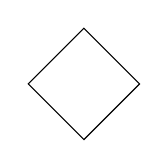
\begin{tikzpicture}[rotate=45]
	\draw (0,0) rectangle (1,1);
\end{tikzpicture}

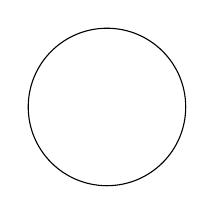
\begin{tikzpicture}[xshift=2cm, yshift=1cm]
	\draw (0,0) circle (1);
\end{tikzpicture}

Texto \begin{tikzpicture}[baseline=-0.5ex]
	\draw (0,0) circle (0.5ex);
\end{tikzpicture} texto

\textbf{3. Comandos Básicos de Dibujo} \\[3mm]
\textbf{3.1. Comando } \verb|\draw|

1 - \verb|\draw (x,y) -- (x,y);|
\textbf{Descripción:} {Ejemplo:}Dibuja una línea recta \verb|\draw (0,0) -- (2,1) -- (3,0);|

\begin{tikzpicture}
\draw (0,0) -- (2,1) -- (3,0);
\end{tikzpicture}

2 - \verb|\draw (x,y) - (x,y);|
Descripción: Línea horizontal luego vertical
Ejemplo: \verb|\draw (0,0) - (2,1);|

\begin{tikzpicture}
\draw (0,0) -| (2,1);
\end{tikzpicture} \\[3mm]

\begin{tikzpicture}
	\draw (0,0) |- (2,1);
\end{tikzpicture}


\begin{tikzpicture}
	\fill[red] (2,0) rectangle (3,1);
\end{tikzpicture}

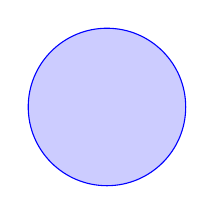
\begin{tikzpicture}
	\filldraw[fill=blue!20, draw=blue] (0,0) circle (1);
\end{tikzpicture}


\begin{tikzpicture}
	\shade[left color=red, right color=blue] (0,0) rectangle (2,1);
\end{tikzpicture} \\[5mm]

\begin{tikzpicture}
	\draw[red] (0,0) -- (1,0);
\end{tikzpicture}

\begin{tikzpicture}
	\draw[draw=blue] (0,-0.5) -- (1,-0.5);
\end{tikzpicture} \\[3mm]

\begin{tikzpicture}
	\draw[color=green!50!black] (0,-1) -- (1,-1);
\end{tikzpicture} \\[3mm]

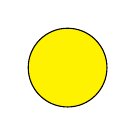
\begin{tikzpicture}
	\draw[fill=yellow] (0,-2) circle (0.5);
\end{tikzpicture} \\[3mm]

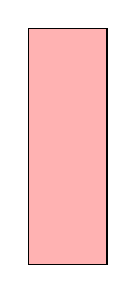
\begin{tikzpicture}
	\draw[fill=red!30] (1,-2) rectangle (2,1);
\end{tikzpicture} \\[3mm]

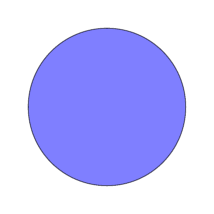
\begin{tikzpicture}
	\draw[fill=blue, opacity=0.5] (0,0) circle (1);
\end{tikzpicture} \\[3mm]

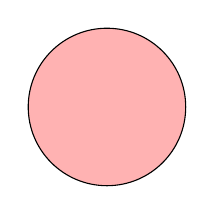
\begin{tikzpicture}
	\draw[fill=red, fill opacity=0.3, draw opacity=1] (0,0) circle (1);
\end{tikzpicture} \\[3mm]

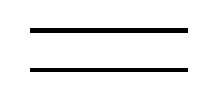
\begin{tikzpicture}
	\draw[line width=2pt] (0,0) -- (2,0);
	\draw[line width=0.5mm] (0,-0.5) -- (2,-0.5);
\end{tikzpicture} \\[3mm]


\begin{tikzpicture}
	\draw[ultra thin] (0,3) -- (1,3);
	\draw[very thin] (0,2.5) -- (1,2.5);
	\draw[thin] (0,2) -- (1,2);
	\draw[semithick] (0,1.5) -- (1,1.5);
	\draw[thick] (0,1) -- (1,1);
	\draw[very thick] (0,0.5) -- (1,0.5);
	\draw[ultra thick] (0,0) -- (1,0);
\end{tikzpicture} \\[3mm]

\begin{tikzpicture}
	\draw[solid] (0,3) -- (2,3);
	\draw[dashed] (0,2.5) -- (2,2.5);
	\draw[dotted] (0,2) -- (2,2);
	\draw[dashdotted] (0,1.5) -- (2,1.5);
	\draw[densely dashed] (0,1) -- (2,1);
	\draw[loosely dashed] (0,0.5) -- (2,0.5);
\end{tikzpicture} \\[3mm]

\begin{tikzpicture}
	\draw[dash pattern=on 2pt off 3pt on 4pt off 4pt] (0,0) -- (3,0);
\end{tikzpicture} \\[3mm]


\begin{tikzpicture}
	\draw[line width=5pt, line cap=rect] (0,1) -- (2,1);
	\draw[line width=5pt, line cap=round] (0,0.5) -- (2,0.5);
	\draw[line width=5pt, line cap=butt] (0,0) -- (2,0);
\end{tikzpicture} \\[3mm]


\begin{tikzpicture}
	\draw[line width=5pt, line join=miter] (0,0) -- (1,1) -- (2,0);
	\draw[line width=5pt, line join=round] (0,0) -- (1,1) -- (2,0);
	\draw[line width=5pt, line join=bevel] (0,0) -- (1,1) -- (2,0);
\end{tikzpicture} \\[3mm]

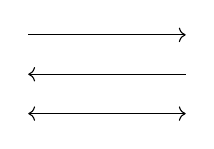
\begin{tikzpicture}
	\draw[->] (0,0) -- (2,0);
	\draw[<-] (0,-0.5) -- (2,-0.5);
	\draw[<->] (0,-1) -- (2,-1);
\end{tikzpicture} \\[3mm]

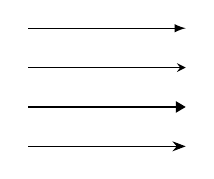
\begin{tikzpicture}
	\draw[-latex] (0,0) -- (2,0);
	\draw[-stealth] (0,-0.5) -- (2,-0.5);
	\draw[-Stealth] (0,-1.5) -- (2,-1.5);
	\draw[-Triangle] (0,-1) -- (2,-1);
\end{tikzpicture} \\[3mm]

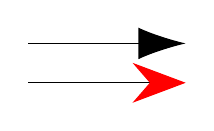
\begin{tikzpicture}
	\draw[-{Latex[length=6mm, width=4mm]}] (0,0) -- (2,0);
	\draw[-{Stealth[red, scale=4]}] (0,-0.5) -- (2,-0.5);
\end{tikzpicture} \\[3mm]


\begin{tikzpicture}
	\node at (0,0) {Texto};
	\node at (0,-.5) {(0,0)};
	\node[red] at (2,0) {Rojo};
	\node[red] at (2,-.5) {(2,-1)};
\end{tikzpicture} \\[3mm]

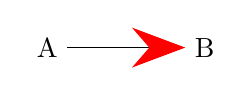
\begin{tikzpicture}
	\node (A) at (0,0) {A};
	\node (B) at (2,0) {B};
	\draw[-{Stealth[red, scale=4]}] (A) -- (B);
\end{tikzpicture} \\[3mm]

\begin{tikzpicture}
	\node[anchor=north] at (0,2) {Norte};
	\node[anchor=south east] at (2,0) {SE};
\end{tikzpicture} \\[3mm]


\begin{tikzpicture}
	\node (A) at (0,0) {A};
	\node[above] at (A) {Arriba de A};
	\node[right=.5cm] at (A) {Derecha de A};
\end{tikzpicture} \\[3mm]

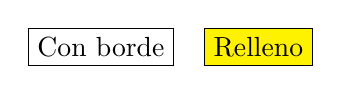
\begin{tikzpicture}
	\node[draw] at (0,0) {Con borde};
	\node[draw, fill=yellow] at (2,0) {Relleno};
\end{tikzpicture} \\[3mm]


\begin{tikzpicture}
	\node[draw, circle] at (0,0) {O};
	\node[draw, rectangle] at (2,0) {R};
	\node[draw, ellipse] at (3.5,0) {Toribio};
\end{tikzpicture} \\[3mm]

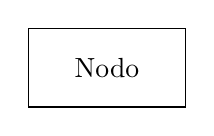
\begin{tikzpicture}
	\node[draw, minimum width=2cm, minimum height=1cm] at (0,0) {Nodo};
\end{tikzpicture} \\[3mm]

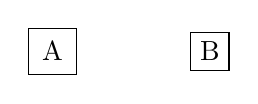
\begin{tikzpicture}
	\node[draw, inner sep=5pt] at (0,0) {A};
	\node[draw, outer sep=10pt] at (2,0) {B};
\end{tikzpicture} \\[3mm]


\begin{tikzpicture}
	\node[draw, text width=3cm] at (0,0) {Texto largo que se ajusta automáticamente};
\end{tikzpicture} \\[3mm]

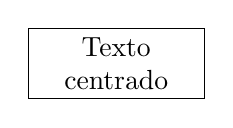
\begin{tikzpicture}
	\node[draw, text width=2cm, align=center] at (0,0) {Texto\\centrado};
\end{tikzpicture} \\[3mm]


\begin{tikzpicture}
	\node[rotate=45] at (0,0) {Rotado};
\end{tikzpicture} \\[3mm]


\begin{tikzpicture}
	\node[font=\Large\bfseries] at (0,0) {Grande y negrita};
	\node[font=\tiny] at (4,0) {Pequeño};
\end{tikzpicture} \\[3mm]

\begin{tikzpicture}
	\draw (0,0) -- (2,1);
	\draw (1cm,2cm) -- (3cm,1cm);
\end{tikzpicture} \\[3mm]

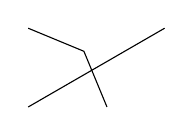
\begin{tikzpicture}
	\draw (0:1) -- (45:1) -- (90:1);
	\draw (0,0) -- (30:2cm);
\end{tikzpicture} \\[3mm]

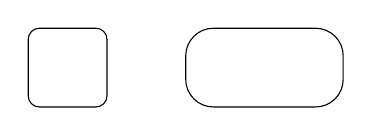
\begin{tikzpicture}
	\draw[rounded corners] (0,0) -- (1,0) -- (1,1) -- (0,1) -- cycle;
	\draw[rounded corners=10pt] (2,0) rectangle (4,1);
\end{tikzpicture} \\[3mm]

\begin{tikzpicture}
	\draw plot coordinates {(0,0) (1,1) (2,0.5) (3,2)};
	\draw[domain=0:6.8] plot (\x, {sin(\x r)});
\end{tikzpicture} \\[3mm]


\begin{tikzpicture}
	\foreach \x in {0,1,2,3}
	\draw (\x,0) circle (0.2);
\end{tikzpicture} \\[3mm]

\begin{tikzpicture}
	\foreach \x/\y in {0/0, 1/1, 2/0.5}
	\fill (\x,\y) circle (2pt);
\end{tikzpicture} \\[3mm]

\begin{tikzpicture}

    \begin{tikzpicture}[scale=0.8]
        % Triángulo
        \draw[thick] (0,0) -- (4,0) -- (4,3) -- cycle;

        % Arco del ángulo
        \draw[blue,thick] (1,0) arc (0:36.87:1);

        % Etiqueta
        \node[blue] at (2,0.4) {$\theta$=36.87};

        % Puntos
        \fill (0,0) circle (2pt);
        \fill (4,0) circle (2pt);
        \fill (4,3) circle (2pt);

        % Líneas guías
        \draw[dashed] (0,0) -- (4,3);
    \end{tikzpicture}


\end{tikzpicture} \\[3mm]

%\begin{tikzpicture}

%\end{tikzpicture} \\[3mm]



\end{document}